\begin{samplecase}
{\bf Fission cross sections: n + ${}^{232}$Th: WKB approach}\newline
This sample case shows the
WKB approximation to calculate fission transmission coefficients as outlined in
Ref. \cite{Sin2006} and Ref. \cite{Goriely2011}. It can be invoked
with the keyword {\bf fismodel 5}.

We use the following input file,

\VerbatimInput{\samples n-Th232-fis-wkb/org/talys.inp}

The above parameters are the usual ones to be adjusted to get good
agreement with experimental data: fission parameters and level density parameters
on top of the barriers.
The resulting file {\em fission.tot} is plotted
together with experimental data in Fig.~\ref{fissioneps-wkb}.

\end{samplecase}
\begin{figure}
\centering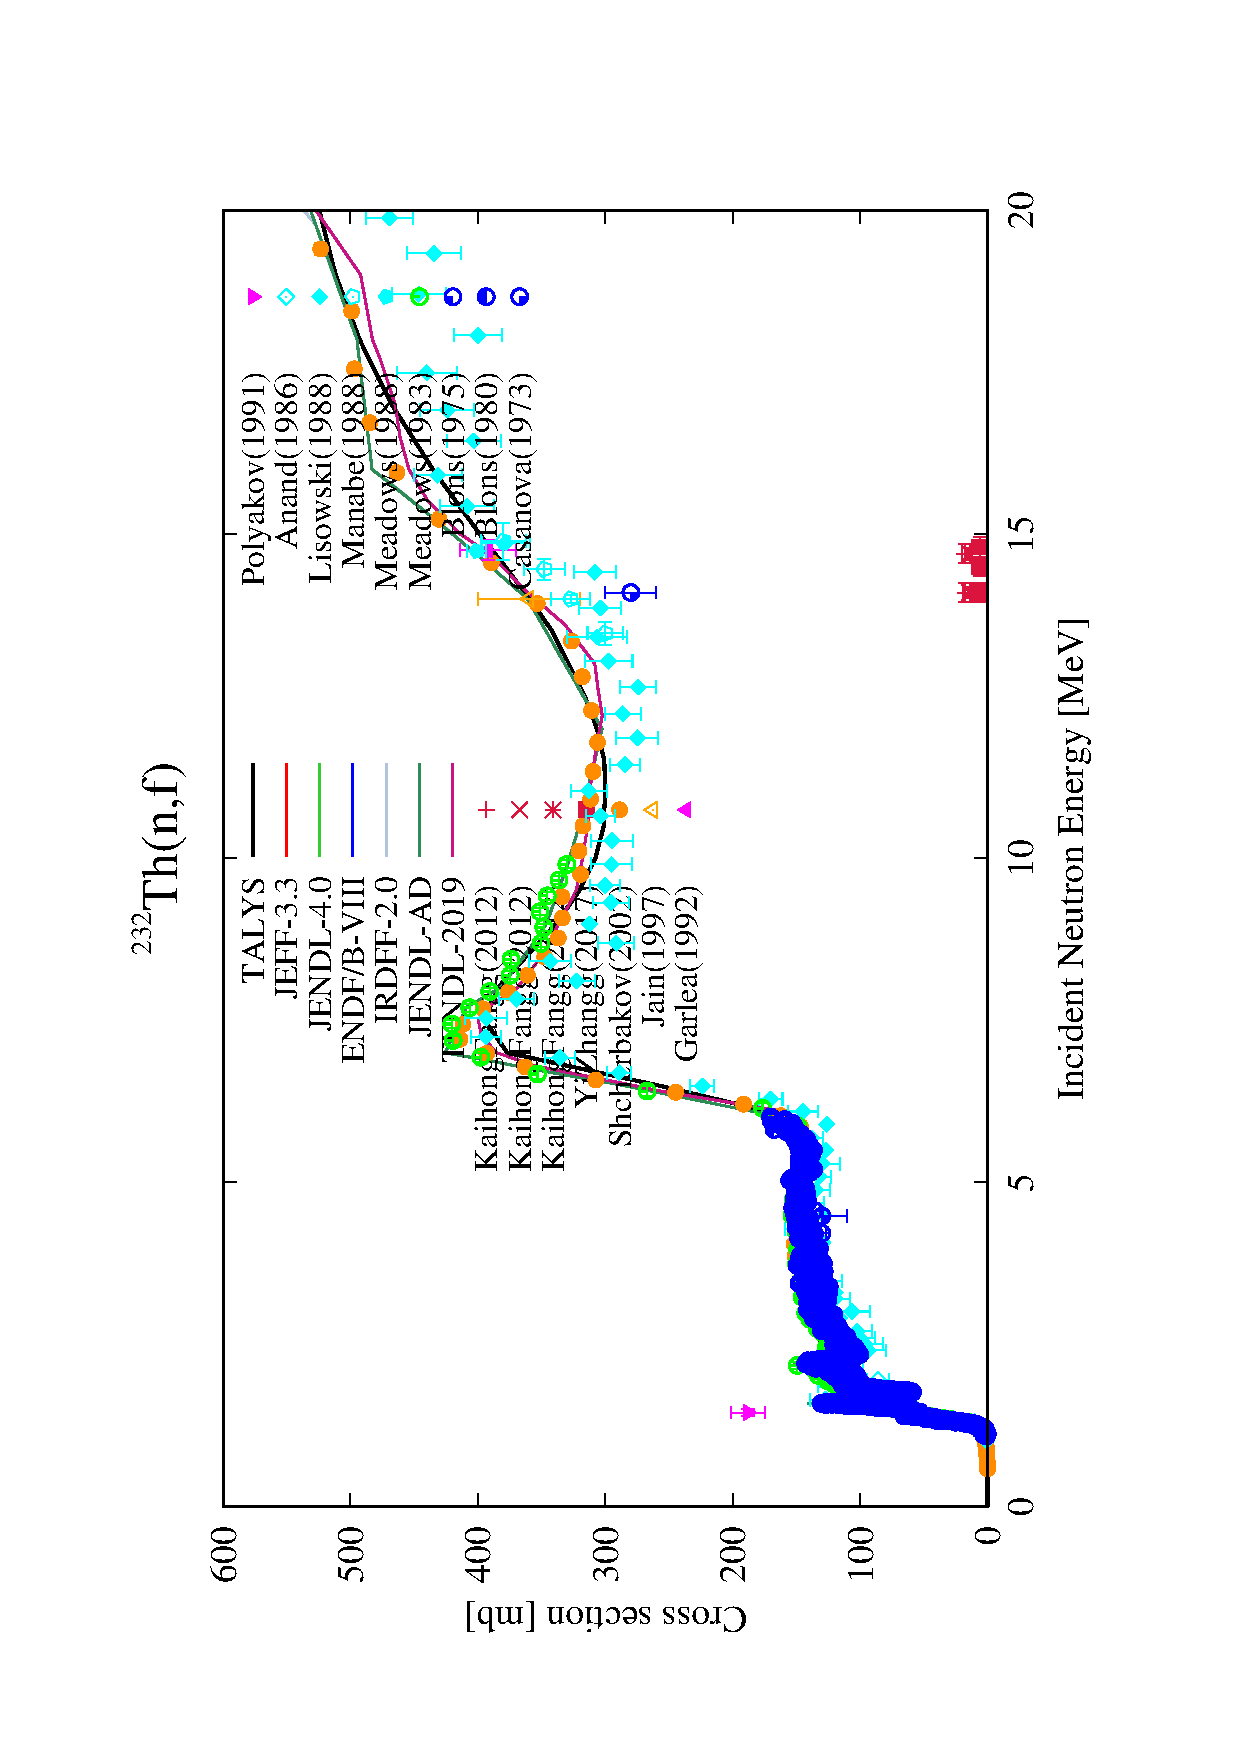
\includegraphics[scale=0.5,angle=270]{n-Th232-fis-wkb}
\caption{Neutron induced fission cross section of ${}^{232}$Th compared with
experimental data. Calculation with fismodel 5 (WKB)}
\label{fissioneps-wkb}
\end{figure}
